\newpage % Rozdziały zaczynamy od nowej strony.
\section{Main Framework}

A causal knowledge graph is not merely a static record of the literature: it can be systematically audited, weighted, and enriched with observational data,
 and subsequently used as the basis for explainable clinical prediction of drug-related outcomes. This thesis operationalizes that idea through two 
 complementary graph neural network tasks, applied to a shared causal knowledge graph of pharmacotherapy:

 \begin{enumerate}[label=\alph*)]
    \item \textbf{Task A:} link prediction, which reconstructs and updates the knowledge graph based on real patient data;
    \item \textbf{Task B:} node classification, which predicts patient-specific clinical endpoints based on the knowledge graph and real patient data.
\end{enumerate}

Since both tasks operate on the same underlying knowledge graph, we adopt graph 
neural networks as the common modeling framework, and enrich them with 
Hierarchical Correlation Reconstruction (HCR). In Figure \ref{fig:architecture} there is presented 
a high-level approach to construct GNN with HCR. While the two tasks share this common foundation, their implementation details differ in several respects; 
we therefore present each task separately in the following subsections.
%moze tutaj damy referencje do Wide&Deep architecture - https://arxiv.org/abs/1606.07792


\begin{figure}[h]
    \centering
    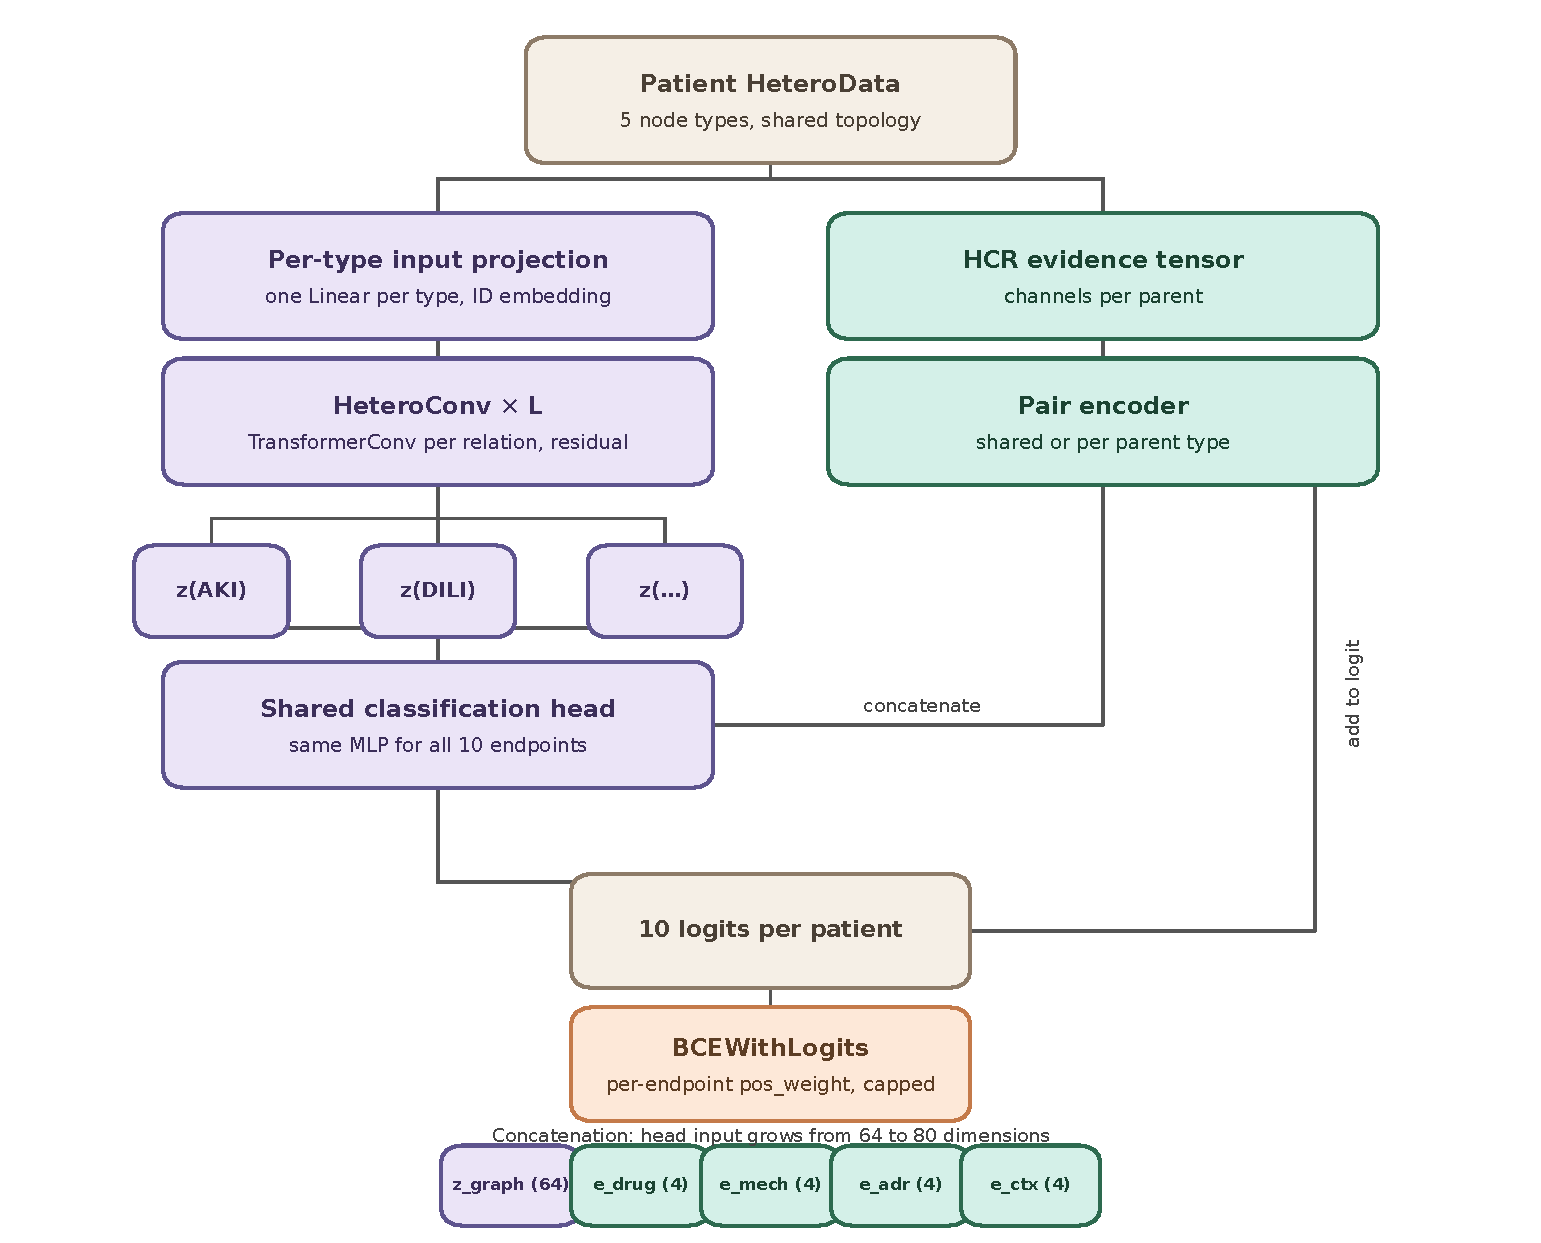
\includegraphics[width=0.95\textwidth,keepaspectratio]{rysunki/architecture_slide_multilabel_hcr.pdf}
    \caption{The presentation of approach to node classification task.}
    \label{fig:architecture}
\end{figure}